\chapter{Twists, Wrenches, and the Screw Axis}
\label{ch:screw_axes}
\label{laymans:context_box}

One rigid displacement can be described by a screw. A moving body generally requires a changing sequence of instantaneous screws. The distinction lets us describe a golf club precisely without assuming that its entire swing follows one fixed axis.

The purpose of this chapter is to connect three questions: where is the body, how is every point on it moving, and how do applied loads do work? A pose answers the first question, a twist the second, and a wrench the third. Their compact notation is useful because it preserves these physical relationships under a change of coordinates. It does not remove the need to specify a body, a reference point, an observer, or a force application point.

We use angular-first twists $V=(\omega,v)^T$ and moment-first wrenches $F=(n,f)^T$. Here $\omega$ is angular velocity, $v$ is the linear coordinate of a rigid velocity field, $n$ is moment about the specified origin, and $f$ is resultant force. Angular velocity is measured in rad/s, linear velocity in m/s, moment in N\,m and force in N. Radians are dimensionless in SI, but retaining rad in pitch units helps distinguish metres per radian from metres per revolution. A six-vector therefore combines components with different physical units; its ordinary Euclidean norm is not automatically a meaningful mechanical magnitude.

\section{Historical Context: From Chasles to Modern Screw Theory}
\label{sec:historical_context_screws}
\label{princ:twist_wrench_convention}

Classical screw theory describes rotations with accompanying translations, and forces with accompanying moments. Ball's treatise \cite{ball1900} is a historical reference; modern robotics texts express related constructions using the Lie group of rigid transformations and its tangent algebra \cite{Murray1994,Lynch2017}. Historical priority is not needed for the derivations below. In particular, a finite-displacement theorem must not be used as if it established a fixed axis for an arbitrary time-dependent motion.

Conventions differ across those references. Murray, Li, and Sastry use linear-first twist coordinates $(v,\omega)$ and force-first wrench coordinates $(f,n)$. Lynch and Park use the angular-first and moment-first ordering adopted here. Featherstone's spatial motion and force vectors also put angular velocity and moment first \cite{Featherstone2008}. These are ordering choices, not different mechanics. If $P$ swaps the two three-component blocks, then $V'=PV$, $F'=PF$ and $F'^T V'=F^T V$; a matrix representing a motion map changes to $PXP^T$. Copying a formula while keeping the wrong vector order changes its meaning.

\begin{figure}[htbp]
\centering
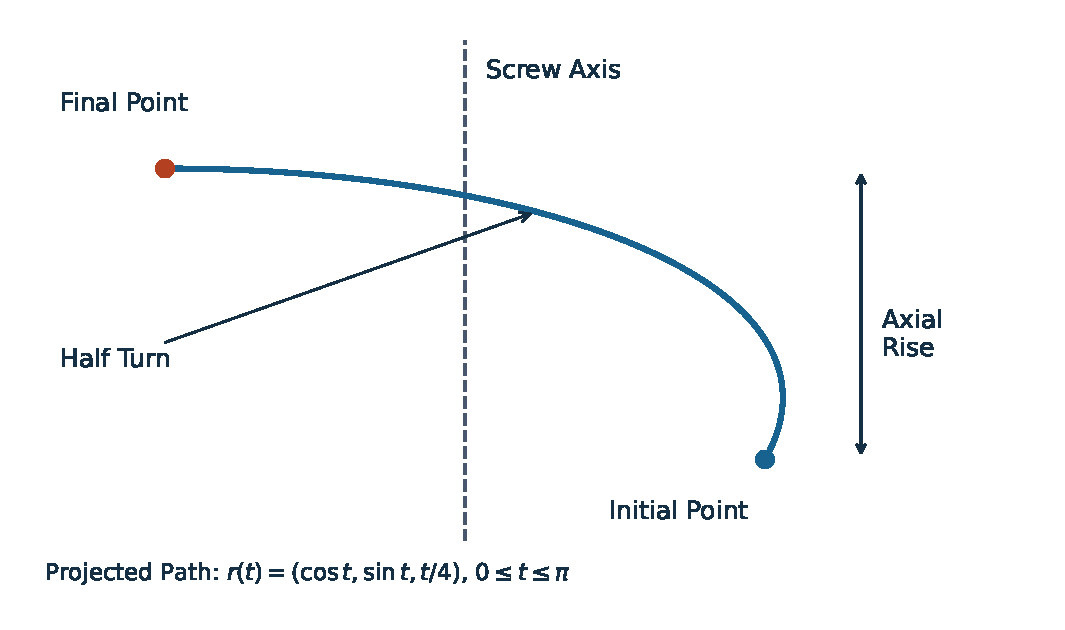
\includegraphics[width=\linewidth]{../figures/screw_displacement.pdf}
\caption{A Constant-Axis Screw Path in Projection. The Point Rotates Through Half a Turn While Rising Along the Axis; the Endpoint Theorem Does Not Require This Particular Intervening Path.}
\label{fig:screw_axis}
\end{figure}

\section{The Unified Four-by-Four Transform SE(3)}
\label{sec:se3_definition}
\label{def:homo_matrix}

Let $T_{AB}$ map coordinates expressed in frame B to coordinates expressed in frame A. Frame B's origin has coordinates $p_{AB}$ in A, and $R_{AB}$ rotates B components into A components. For a point and a free direction, respectively,
\begin{equation}
 x_A=R_{AB}x_B+p_{AB},\qquad d_A=R_{AB}d_B.
\end{equation}
Translation is affine on three-dimensional point coordinates: it does not preserve the zero vector. No principle of linear algebra is violated. Homogeneous coordinates embed points with weight one and directions with weight zero:
\begin{equation}
 T_{AB}=\begin{bmatrix}R_{AB}&p_{AB}\\0&1\end{bmatrix},\qquad
 \begin{bmatrix}x_A\\1\end{bmatrix}=T_{AB}\begin{bmatrix}x_B\\1\end{bmatrix},\qquad
 \begin{bmatrix}d_A\\0\end{bmatrix}=T_{AB}\begin{bmatrix}d_B\\0\end{bmatrix}.
\end{equation}
The set $SE(3)$ consists of these matrices with $R^TR=I$ and $\det R=1$. Reflections, arbitrary scale changes and finite Euler approximations to rotations are not generally in this set. Separate arrays for rotation and translation are equally legitimate implementations; a homogeneous matrix is a representation, not a requirement imposed on every physics engine.

\subsection{Group Structure of SE(3)}
\label{subsec:se3_group_structure}
\label{thm:se3_lie_group}
\label{princ:se3_composition}

Following the frame subscripts gives composition and inversion:
\begin{equation}
 T_{AC}=T_{AB}T_{BC},\qquad
 T^{-1}=\begin{bmatrix}R^T&-R^Tp\\0&1\end{bmatrix}.
\end{equation}
The product has rotation $R_1R_2$ and translation $p_1+R_1p_2$, so it remains a proper rigid transform. Identity and inverses belong to the set, and associativity follows from matrix multiplication. The parameters form a smooth six-dimensional manifold: three local rotational coordinates and three translations. Multiplication and inversion are smooth, making $SE(3)$ a Lie group. Six-dimensional does not mean that one nonsingular three-angle chart covers all rotations; rotation charts still have their familiar limitations.

Composition order matters. Rotating a club and then translating it by a vector fixed in the laboratory is generally a different operation from translating it and then rotating about the laboratory origin. Subscripts and the point-mapping equation are safer guides than an unexplained instruction to ``premultiply'' or ``postmultiply.''

\section{Chasles' Theorem and the Screw Axis}
\label{sec:chasles_theorem}
\label{def:screw_params}
\label{ex:football_frisbee}
\label{laymans:screwaxis}
\label{thm:chasles}

Consider a finite displacement $x'=Rx+p$ in one common spatial coordinate system. If $R$ is not identity, this displacement can be realized as a rotation about a line, followed by a translation parallel to that line. Choose a unit direction $s$ and a principal angle $0<\theta\leq\pi$ with $R=\exp([s]_\times\theta)$. There are a point $q$ on the line and an axial displacement $d$ such that
\begin{equation}
 x'=q+R(x-q)+ds,\qquad p=(I-R)q+ds.
\end{equation}
Every point $q+\lambda s$ on the axis moves to $q+(\lambda+d)s$. Other points have a rotational displacement around the line as well as the axial displacement. The signed finite pitch is $h=d/\theta$, not $d$ and not the total distance travelled by an off-axis point divided by angle.

This is an endpoint statement. If a tracked body has poses $T_0$ and $T_1$ relative to the same laboratory frame, the spatial displacement mapping each initial material-point position to its final position is $\Delta T=T_1T_0^{-1}$. Decomposing $T_1$ alone instead describes a mapping from the chosen body reference coordinates. It generally gives a different axis. The corresponding body-coordinate relative transform is $T_0^{-1}T_1$; its coordinates must be interpreted accordingly.

\subsection{Geometric Description and Exceptional Cases}

The axis line is $\{q+\lambda s:\lambda\in\mathbb R\}$. Replacing $q$ by $q+\lambda s$ does not change the line. We normally choose its closest point to the origin, $q\cdot s=0$. For nonidentity $R$, this geometric line is unique. Its oriented parameterization has branch qualifications: at a half turn, $s$ and $-s$ represent the same rotation, while the signed axial coordinate and pitch change with that choice. Additional full turns also produce alternative angle/pitch descriptions of the same endpoints.

For pure translation, $R=I$ and $p\ne0$, every line parallel to $p$ can serve as a translational axis. There is no unique finite rotational axis or finite pitch obtained by dividing by a zero angle. Calling this ``infinite pitch'' is a limiting convention, not an instruction to divide by zero. Identity displacement has neither a preferred axis nor a required nonzero motion. An object can even execute a nontrivial closed path and return to identity displacement: its endpoints alone do not reconstruct that path.

A steadily advancing ideal screw provides a useful constant-axis example. A tumbling football or precessing frisbee generally does not. Each instantaneous rigid velocity field and each nontrivial finite relative pose has its own appropriate screw description; those descriptions need not coincide over a measured time interval. This distinction is especially relevant when a changing swing plane is inferred from a sequence of club poses.

\section{The Spatial Twist}
\label{sec:spatial_twist}
\label{def:se3_algebra}
\label{ex:joint_twists}
\label{def:spatial_twist}

Let $T(t)$ give the moving body's pose in a fixed laboratory frame. Differentiating $T$ produces a tangent matrix at $T$, not directly a six-vector at identity. Two useful representations are
\begin{equation}
 \widehat V_s=\dot T T^{-1},\qquad \widehat V_b=T^{-1}\dot T,
 \qquad \widehat V=\begin{bmatrix}[\omega]_\times&v\\0&0\end{bmatrix}.
\end{equation}
\label{eq:se3_matrix}
\label{eq:twist_def}
The subscripts denote spatial and body representations of the same body motion relative to the laboratory. With $T=(R,p)$, direct multiplication gives
\begin{equation}
 [\omega_s]_\times=\dot R R^T,\quad v_s=\dot p-\omega_s\times p,
 \qquad [\omega_b]_\times=R^T\dot R,\quad v_b=R^T\dot p.
\end{equation}
In particular, $v_s$ is not generally the velocity $\dot p$ of the body-frame origin. It is the velocity assigned by the body's rigid velocity field to the point located at the spatial origin. That point need not lie inside the physical body. The spatial field evaluated at any material point with current position $r$ is
\begin{equation}
 u(r)=v_s+\omega_s\times r.
\end{equation}
For $r=p+Rx_b$ with fixed material coordinates $x_b$, this equals $\dot p+\dot R x_b$, as it must. This identity is an immediate way to check a twist convention against measured marker velocities.

\subsection{Screw Representation of a Twist}

When $\omega\ne0$, set $s=\omega/\|\omega\|$, choose rate $\dot\theta=\|\omega\|$, and define
\begin{equation}
 h=\frac{\omega\cdot v}{\|\omega\|^2},\qquad
 q=\frac{\omega\times v}{\|\omega\|^2},\qquad
 V=S\dot\theta,\quad S=\begin{bmatrix}s\\q\times s+hs\end{bmatrix}.
\end{equation}
\label{eq:screw_coordinates}
The vector identity $\omega\times(\omega\times v)=\omega(\omega\cdot v)-\|\omega\|^2v$ verifies the formula. Every point on this instantaneous axis has velocity $h\omega$; off-axis points have an additional rotational contribution. Thus pitch uses the axial projection of velocity, not $\|v\|/\|\omega\|$ and not clubhead speed divided by angular speed. With an independently chosen oriented joint axis, $\dot\theta$ may instead be signed.

The phrase ``unit screw'' here means $\|s\|=1$ in the angular block for a rotational joint. It does not mean $\|S\|=1$ under an arbitrary mixed-unit six-dimensional norm. For pure translation, $\omega=0$ and $v\ne0$, one can use $S=(0,s)$ with $\|s\|=1$ and a translational joint coordinate in metres. The zero twist does not determine an instantaneous axis.

\subsection{Twists for Standard Joint Types}

A revolute joint through $q$ in direction $s$ has $S=(s,q\times s)$ and zero pitch. The linear block is not zero merely because points on the axis are instantaneously stationary: their complete velocity is $q\times s+s\times q=0$ for unit angular rate. A prismatic joint has $S=(0,s)$, and a helical joint has $S=(s,q\times s+hs)$. These are relative joint twists. In a moving mechanism, an absolute link twist also includes the predecessor's motion, expressed in a common frame.

For an axis through $(1,0,0)$ parallel to $z$, take $h=2$ m/rad and rate $0.5$ rad/s. The twist is $V=(0,0,0.5,0,-0.5,1)^T$. At the axis point, $u(q)=(0,0,1)$ m/s; at the origin, $u(0)=(0,-0.5,1)$ m/s. Both velocities belong to the same rigid field. A zero-pitch revolute joint at that location would retain the $-0.5$ linear component but have zero velocity at $q$.

\subsection{Matrix Representation and Finite Integration}

The matrices $\widehat V$ form the Lie algebra $\mathfrak{se}(3)$. Only the upper-left rotational block is skew-symmetric; the full four-by-four matrix is generally not. Differentiating $R^TR=I$ explains that skew-symmetry. The translation column is unrestricted and the last row is zero, leaving six independent coordinates.

For a constant spatial twist, $\dot T=\widehat V_sT$ integrates to $T(t)=\exp(\widehat V_st)T(0)$. For a constant body twist, $\dot T=T\widehat V_b$ integrates to $T(t)=T(0)\exp(\widehat V_bt)$. For a general time-dependent twist, successive increments require their correct order. Replacing them by the exponential of the simple time integral is justified only under additional commutation conditions. A single fitted endpoint screw does not show that the intervening twist was constant.

\subsection{The Lie Bracket of Twists}

The matrix commutator induces the angular-first bracket
\begin{equation}
 [V_1,V_2]=\begin{bmatrix}
 \omega_1\times\omega_2\\
 \omega_1\times v_2-\omega_2\times v_1
 \end{bmatrix}.
\end{equation}
It describes the leading second-order effect of changing the order of small transformations. With the stated matrix order,
\begin{equation}
 e^{\epsilon\widehat V_1}e^{\epsilon\widehat V_2}
 e^{-\epsilon\widehat V_1}e^{-\epsilon\widehat V_2}
 =I+\epsilon^2[\widehat V_1,\widehat V_2]+O(\epsilon^3).
\end{equation}
The bracket is not simply the relative velocity $V_1-V_2$. Its role becomes important when rotations at different joints or times do not commute. It provides a local geometric description, not by itself a prediction of a finite golf-swing outcome.

\section{The Adjoint Representation}
\label{sec:adjoint}
\label{def:adjoint_definition}

\subsection{Changing Reference Frames}

Suppose A and B are two coordinate frames used to represent the same physical velocity field. At the instant of interest, $x_A=Rx_B+p$ with $T_{AB}=(R,p)$. Substituting the point-velocity fields gives
\begin{equation}
 \omega_A=R\omega_B,\qquad v_A=Rv_B+p\times R\omega_B.
\end{equation}
The angular-first adjoint is therefore
\begin{equation}
 V_A=X V_B,\qquad X=\operatorname{Ad}_{T_{AB}}
 =\begin{bmatrix}R&0\\{}[p]_\times R&R\end{bmatrix}.
\end{equation}
\label{eq:adjoint}
Equivalently, $\widehat V_A=T_{AB}\widehat V_BT_{AB}^{-1}$. To check the sign of the offset term, evaluate $u_A(Rr_B+p)$: the $p\times R\omega_B$ term cancels the $R\omega_B\times p$ from point evaluation, leaving $Ru_B(r_B)$. Also $\operatorname{Ad}_{T_1T_2}=\operatorname{Ad}_{T_1}\operatorname{Ad}_{T_2}$ by matrix conjugation. For the moving body's pose, $V_s=\operatorname{Ad}_T V_b$ follows from the two derivative definitions above.

Re-expression must be distinguished from changing the physical observer. If A and B themselves move relative to each other, differentiating point coordinates gives extra frame-motion terms:
\begin{equation}
 \dot x_A=R\dot x_B+\dot R x_B+\dot p.
\end{equation}
The adjoint re-expresses a specified relative motion; it does not automatically subtract an observer's own velocity. In particular, body representation $V_b$ still describes body motion relative to the laboratory, even though the body's material coordinates are constant. A calculation of motion relative to another moving body must first specify that relative motion and then express it in the chosen frame.

\section{The Spatial Wrench}
\label{sec:spatial_wrench}
\label{def:wrench_dual}
\label{def:spatial_wrench}

A collection of forces $f_i$ applied at positions $r_i$ and free couples $c_i$, all expressed in one frame, has resultant wrench about that frame's origin
\begin{equation}
 F=\begin{bmatrix}n\\f\end{bmatrix},\qquad
 f=\sum_i f_i,\quad n=\sum_i(r_i\times f_i+c_i).
\end{equation}
\label{eq:wrench_def}
A couple has a moment independent of the chosen origin; the moment of a nonzero resultant force generally changes with origin. Wrenches form the dual space $\mathfrak{se}(3)^*$ under the power pairing. A list of six components is not a reason to identify a wrench with a twist in $\mathfrak{se}(3)$. The distinction fixes the correct transformation law.

\subsection{Wrenches From Forces and Moments}

A force $(f_x,0,0)$ applied at $(0,0,d)$ produces moment $(0,df_x,0)$, with positive $y$ sign for positive $d$ and $f_x$. Moving the same force along its line of action leaves its moment unchanged. A force $(1,0,0)$ N at $(0,2,0)$ m instead gives $n=(0,0,-2)$ N\,m. These elementary cross products are useful checks on any six-dimensional formula.

\subsection{Wrench Transformation Under Changes of Frame}

For the same B-to-A transform used for motion,
\begin{equation}
 f_A=Rf_B,\qquad n_A=Rn_B+p\times Rf_B,
 \qquad F_A=X^{-T}F_B.
\end{equation}
The reverse mapping is $F_B=X^TF_A$. Thus a transpose alone is correct when converting an A wrench to B, while $X$ converts a B twist to A. Applying $X$ and $X^T$ in the same B-to-A direction is generally wrong. One can derive the force rule directly by writing $r_A=Rr_B+p$ and $f_A=Rf_B$ in $r_A\times f_A$, or derive it from $F_A^TV_A=F_B^TV_B$ for every $V_B$. Both derivations agree.

\subsection{Physical Interpretation of Wrenches: Forces and Torques Unified}
\label{sec:wrench_physical_interpretation}
\index{screw!pitch}
\index{pure force}
\index{pure couple}
\index{force at offset}
\index{dual space}
\index{Wrench!pure force}
\index{Wrench!pure couple}
\index{Wrench!offset force}
\index{Wrench!geometric object}
\label{laymans:wrench_unified_motivation}
\label{ex:canonical_wrenches}
\index{Wrench!physical interpretation}

The wrench is a compact account of a body's resultant load, not a specification of how that load is distributed across skin, fingers, shafts or individual contacts. Different grip pressure distributions can have the same net wrench while producing different local stress or friction margins. Likewise, a wrench axis is not generally the instantaneous axis of the body on which it acts. Motion also depends on inertia, initial state and constraints.

For $f\ne0$, the wrench's central axis and signed pitch are
\begin{equation}
 q_F=\frac{f\times n}{\|f\|^2},\qquad h_F=\frac{f\cdot n}{\|f\|^2},
 \qquad n=q_F\times f+h_F f.
\end{equation}
The cross-product identity verifies this decomposition. On that line the remaining moment is parallel to the resultant force. A pure force has $h_F=0$, although its moment about a remote origin may be nonzero. A pure couple has $f=0$ and no unique finite central line; an ``infinite-pitch wrench'' is again a convention. The zero wrench has no distinguished line. Although both pitches have dimensions of length when radians are suppressed, $h_F$ and the motion pitch $h$ describe different objects and need not be equal.

\section{Proof of Chasles' Theorem}
\label{sec:chasles_proof}
\label{laymans:chasles_one_sentence}
\label{thm:chasles_formal}
\index{Chasles' theorem!proof}

Here is a constructive proof. A proper rotation with $R\ne I$ has an invariant unit direction $s$ and rotates its perpendicular plane by a nonzero angle modulo $2\pi$. Resolve the displacement and define its pitch as
\begin{equation}
 d=s^Tp,\qquad p_\perp=p-ds,\qquad h=d/\theta.
\end{equation}
\label{eq:chasles_pitch}
Because $s^T(I-R)=0$, any solution of $p=(I-R)q+ds$ must have this axial displacement. Restricted to $s^\perp$, the map $I-R$ is invertible. Choose $q\perp s$ and solve
\begin{equation}
 (I-R)q=p_\perp,\qquad
 q=\frac12p_\perp+\frac12\cot(\theta/2)\,s\times p_\perp.
\end{equation}
\label{eq:chasles_axis_point}
To verify the inverse, put $Jx=s\times x$ on the perpendicular plane, where $J^2=-I$. Rodrigues' formula there is $R=\cos\theta I+\sin\theta J$. Multiplying $[(1-\cos\theta)I-\sin\theta J]$ by $\tfrac12[I+\cot(\theta/2)J]$ gives $I$. This proves the displayed expression, including its cross-product sign. There is no additional cross product outside the restricted inverse.

The resulting $q$ satisfies $p=(I-R)q+ds$, proving the screw representation. Adding any multiple of $s$ gives the same axis line; no other perpendicular point solves the equation. At $\theta=\pi$, the cotangent vanishes and $q=p_\perp/2$, while the direction-sign qualification remains. As $\theta\to0$, the inverse has scale $1/|\theta|$. A small measured perpendicular translation error can therefore produce a large axis-location error. A numerically reported distant axis near pure translation need not indicate a meaningful anatomical pivot.

For a rotation by $\pi/2$ about the vertical line through $(1,0,0)$ followed by $0.2$ m of axial translation, $R=R_z(\pi/2)$ and $p=(1,-1,0.2)$. The formulas give $q=(1,0,0)$, $d=0.2$ m and $h=0.4/\pi\approx0.12732$ m/rad. Substituting a point on and off the axis verifies both endpoints. This finite pitch does not determine elapsed time or the work required to realize the displacement.

\section{Mechanical Work and the Virtual Power Principle}
\label{sec:virtual_power}
\index{power!inner product}
\index{mechanical power}
\index{frame invariance!power}
\index{duality!wrench-twist}
\label{princ:virtual_work}

For loads acting on one rigid body, substitute the velocity field into the sum of physical powers:
\begin{equation}
 P=\sum_i\{f_i\cdot[v+\omega\times r_i]+c_i\cdot\omega\}
 =f\cdot v+n\cdot\omega=F^TV.
\end{equation}
\label{eq:power}
\label{eq:wrench_twist_power}
\label{eq:wrench_twist_pairing}
The scalar triple-product identity converts $f_i\cdot(\omega\times r_i)$ into $(r_i\times f_i)\cdot\omega$. This derivation explains why force and moment must share a reference convention with the twist. Evaluating the linear part at the center of mass while leaving the moment about the grip would omit or double-count a term.

For an admissible virtual generalized velocity $\delta\dot q$, suppose the relevant relative twist is $J\delta\dot q$. Then virtual power is $F^TJ\delta\dot q=(J^TF)^T\delta\dot q$, so the corresponding generalized force is $J^TF$. This is a kinematic duality statement; a dynamic acceleration calculation additionally requires mass, bias terms and constraints. Work over a finite interval is $\int F(t)^TV(t)\,dt$. A single instantaneous positive, negative or zero power does not determine that integral.

\subsection{Invariance of Power and Its Limits}

For a coordinate re-expression of the same motion and load, $F_A^TV_A=(X^{-T}F_B)^TXV_B=F_B^TV_B$. This is a scalar representation identity, not conservation of energy. Under a Galilean change to an observer translating with constant velocity $U$, point velocities become $u_i'=u_i-U$ and the applied-force power becomes $P'=P-f\cdot U$. A rotating observer introduces its own rotational terms. Energy balances must include the chosen observer and system boundary consistently; numerical equality under an adjoint change does not erase those physical choices.

\section{Reciprocal Screws and Constraint Analysis}
\label{sec:reciprocal_screws}
\label{princ:constraint_principle}
\label{def:reciprocal_screws}

A wrench $F$ is reciprocal to a twist $V$ when $F^TV=0$. For a subspace of admissible relative twists $\mathcal T$, ideal reaction wrenches lie in its annihilator: every $F$ in that set satisfies $F^TV=0$ for every $V\in\mathcal T$. If $\mathcal T$ has dimension $d$ within the six-dimensional relative twist space, its annihilator has dimension $6-d$. This is a local linear statement at a specified configuration, not an automatic count of whole-mechanism mobility.

For a spatial revolute joint through $q$ with direction $s$, the condition is
\begin{equation}
 s\cdot(n-q\times f)=0.
\end{equation}
It excludes a reaction moment along the free rotational direction when moments are taken about the joint point. A motor or friction torque in that direction can perform relative work and is not part of the ideal reaction subspace. For a frictionless prismatic joint, $s\cdot f=0$ excludes reaction force along the sliding direction; other spatial reaction components remain possible.

\subsection{Two Geometric Screws and the Reciprocal Product}

When both screws are represented in the same motion-style ordering, the corresponding reciprocal bilinear form is the cross-block expression
\begin{equation}
 B(S_1,S_2)=\omega_1\cdot v_2+v_1\cdot\omega_2.
\end{equation}
This is not their ordinary Euclidean six-vector dot product. A wrench along the geometric screw encoded as $(\omega_2,v_2)$ has its force and moment roles interchanged, yielding moment-first coordinates proportional to $(v_2,\omega_2)$. Screw magnitudes and units must be supplied to interpret the resulting pairing as physical power. The geometric reciprocal product alone is not the power of two velocities.

For zero-pitch normalized axes with directions $s_1,s_2$ through $q_1,q_2$, substitution gives
\begin{equation}
 B=(q_1-q_2)\cdot(s_1\times s_2).
\end{equation}
Thus intersecting, parallel and coincident zero-pitch axes are reciprocal in this geometric sense; perpendicularity is not the defining condition. For finite pitches, add $(h_1+h_2)s_1\cdot s_2$. Constraint analysis must use the correct pairing and actual admissible motions, rather than a visual claim that the axes look orthogonal.

\section{Physical Interpretation of Wrenches}
\label{sec:wrench_physical}
\label{ex:gravity_wrench}
\label{laymans:wrench_unified}

\subsection{Three Fundamental Wrench Types}

A pure couple, a force on a line, and a force plus a parallel couple cover the central-axis cases above. For example, with gravity vector $g=(0,0,-g_0)$, mass $m$, and center-of-mass position $r_C=(a,b,c)$, the gravity wrench about the origin is
\begin{equation}
 F_g=\begin{bmatrix}-mg_0b\\mg_0a\\0\\0\\0\\-mg_0\end{bmatrix}.
\end{equation}
Its moment vanishes when taken about the center of mass, but generally not about a grip or a joint. Summing gravity wrenches for separate bodies requires a common origin and frame, and summing them does not replace each body's dynamic balance.

\subsection{The Wrench--Twist Duality at a Golf Grip}

For hand forces $f_i$ and couples $c_i$ acting on the club at grip locations $r_i$, the club-side hand power is
\begin{equation}
 P_{\rm hands\to club}=\sum_i[f_i\cdot u_{\rm club}(r_i)+c_i\cdot\omega_{\rm club}].
\end{equation}
The same value follows from summing the hand wrenches about any one chosen origin and pairing with the club twist represented there. This is useful when comparing a clubhead-speed narrative with measured grip loads: an angular moment term and a translational force term must be interpreted together. A change in their separate numerical values after moving the origin is not evidence of a different physical energy-transfer mechanism.

If the grip is rigid and no slip occurs, equal-and-opposite interface wrenches have zero total interface power on the combined hand--club system, because their relative twist is zero. Nevertheless either subsystem can receive nonzero power from the other. With compliance or slip, the summed interface power depends on the relative motion and may represent elastic storage or dissipation. The sign must be tied to which body's load and relative velocity are used. A measured net club wrench cannot uniquely identify each hand's contribution or a neural control objective. Those claims require additional measurements and a specified contact and musculoskeletal model.

\subsection{Transforming Wrenches Between Frames}

A practical audit therefore records the sensor orientation, the point about which its moment is reported, the direction of the reported action, and the body-relative motion being paired with it. Transform all simultaneous loads to one frame and origin before adding them. The inverse-transpose rule then does the bookkeeping faithfully. It does not infer an unmeasured grip offset, calibrate a sensor, or separate muscle work from tendon storage.

\section{Wrench Analysis and Force Polytopes}
\label{sec:wrench_analysis}
\label{ex:graphical_statics}

An ideal bilateral reaction subspace is usually unbounded. A unilateral frictionless point contact instead permits $f=\lambda n_c$ with $\lambda\geq0$ along a contact normal. With isotropic Coulomb friction, a common admissibility model is $f_n\geq0$ and $\|f_t\|\leq\mu f_n$. This is a cone; its circular boundary is not a finite-sided polyhedral cone unless approximated. Sliding friction additionally constrains force direction relative to slip velocity. A bounded actuator/contact model can yield a convex polytope, but bounds must actually be supplied. These sets should not be conflated under the word ``polytope.''

If admissible contact variables $\lambda$ produce a resultant wrench $G\lambda$, static support of one free body requires $G\lambda+F_{\rm ext}=0$. The support set must contain $-F_{\rm ext}$, not merely the external load with unchanged sign. Linkages additionally require the internal action--reaction relationships and equilibrium of every link. For moving bodies, a nonzero inertial wrench replaces the zero right-hand side. Neither convexity nor a force polygon removes those balances.

For a concrete bounded example, two vertical bilateral force actuators act on one planar rigid bar at $(0,0)$ and $(L,0)$, with $|u_1|,|u_2|\leq F_{\max}$. In coordinates $(n_z,f_y)$,
\begin{equation}
 (n_z,f_y)=(Lu_2,u_1+u_2),\quad
 |n_z/L|\leq F_{\max},\quad |f_y-n_z/L|\leq F_{\max}.
\end{equation}
For $L=1$ m and $F_{\max}=10$ N, the vertices are $(-10,-20)$, $(10,0)$, $(10,20)$ and $(-10,0)$, with moment in N\,m and force in N. A downward 15 N load at the midpoint requires $(n_z,f_y)=(7.5,15)$ and is feasible with $u_1=u_2=7.5$ N. A downward 25 N load there exceeds the total force capacity. If the two supports can only push upward, replace the bounds by $0\leq u_i\leq F_{\max}$; the feasible set changes. This example concerns two external supports on one body, not two unspecified joints in an arbitrary mechanism.

\section{Worked Example: Planar Four-Bar Statics}
\label{sec:planar_mechanism_example}

\subsection{Setup}

Use a deliberately idealized planar mechanism with ground points $A=(0,0)$ and $D=(4,0)$, moving joints $B=(1,1)$ and $C=(3,1)$, all coordinates in metres. Links AB, BC and CD are rigid and massless; all pins are frictionless. A downward load $(0,-W)$ acts at $E=(x_E,1)$ on the coupler BC. Ground AD is fixed. A motor at A may apply a counterclockwise torque $\tau_A$ to AB; B, C and D are passive pins. The numerical example uses $W=100$ N. Link weight, out-of-plane loading, friction, compliance and acceleration are omitted by assumption.

\subsection{Twist Space of Each Joint}

A planar pin at $q=(q_x,q_y)$ permits the relative angular-first twist
\begin{equation}
 S_q=(0,0,1,q_y,-q_x,0)^T.
\end{equation}
Its reduced planar coordinates are $(\omega_z,v_x,v_y)=(1,q_y,-q_x)$. Pairing with reduced wrench $(n_z,f_x,f_y)$ gives
\begin{equation}
 n_z+q_yf_x-q_xf_y=0,\qquad n_z=q_xf_y-q_yf_x.
\end{equation}
Thus an ideal planar pin transmits arbitrary in-plane force but no independent couple about the pin. Force becomes directed along a link only if that link is an unloaded two-force member. CD has that property here. AB has it only when $\tau_A=0$. The planar model does not prove that a physical spatial bearing lacks out-of-plane reactions; it has excluded those components from its idealization.

\subsection{Constraint Wrenches and Separate Free Bodies}

Let $b=(b_x,b_y)$ and $c=(c_x,c_y)$ be forces on the coupler at B and C. The forces on the side links at those joints are $-b$ and $-c$. Since each side link has no other force, the ground reactions on AB and CD are $b$ at A and $c$ at D. Moment balance for CD about D and for BC about B gives
\begin{equation}
 c_x+c_y=0,\qquad 2c_y-(x_E-1)W=0.
\end{equation}
Coupler force balance and AB moment balance then give
\begin{equation}
 b+c+(0,-W)=0,\qquad \tau_A=b_y-b_x.
\end{equation}
The unit lever-arm factors in the last equation are one metre; the preceding factor two is the two-metre coupler span. These equations retain consistent force and moment units. They are balances of three different bodies, not a sum of all joint forces assigned to one coupler.

\subsection{Equilibrium and the Role of Actuation}

Solving gives
\begin{equation}
 c_y=\frac{(x_E-1)W}{2},\quad c_x=-c_y,\quad
 b_x=c_y,\quad b_y=W-c_y,\quad \tau_A=W(2-x_E).
\end{equation}
Here numerical lengths are in metres and $\tau_A$ is in N\,m. For the centered load $x_E=2$ m, $b=(50,50)$ N, $c=(-50,50)$ N and $\tau_A=0$. Both side links are two-force members. Their lines of force meet at $(2,2)$, on the external load's vertical line of action. The coupler's force polygon closes, and its moment balance is satisfied. This is passive equilibrium at the specified configuration, not a proof of stability against perturbations.

For $x_E=2.5$ m, $b=(75,25)$ N, $c=(-75,75)$ N and $\tau_A=-50$ N\,m. AB is no longer a two-force member because of the motor couple. Removing that required motor torque leaves no static equilibrium for this load at this configuration under the stated assumptions. The external forces still sum to zero; that condition alone is insufficient. For the entire assembly, the moment balance about A is $4c_y+\tau_A-Wx_E=0$, which independently confirms the result.

\subsection{Geometric Interpretation and Virtual Power}

Set the instantaneous angular speed of AB to one rad/s. Then $u_B=(-1,1)$ m/s. Constant length BC requires $u_{C,x}=u_{B,x}$, while CD's pin motion gives $u_C=(-1,-1)$ m/s. Consequently $\omega_{BC}=-1$ rad/s and $u_{E,y}=2-x_E$ m/s. Ideal pin reactions contribute zero net relative power, so static virtual power requires
\begin{equation}
 \tau_A-W(2-x_E)=0.
\end{equation}
This reproduces the free-body torque. At the centered load, the load point's admissible instantaneous motion is horizontal, so the vertical force does no virtual work. The mechanism still has an admissible motion; load reciprocity does not make it rigid. Near other configurations, the relevant constraint or actuation matrices may lose rank and their force solution may become nonunique or infeasible. Geometry, allowed inputs and the actual external load must all be specified before interpreting a mechanism's apparent force-transmission advantage.

\section{Python Implementation}
\label{sec:python_screws}

The companion implementation checks proper rigid transforms and uses angular-first vectors throughout. It exposes the transform direction in the wrench function name and computes the inverse-transpose action by solving a linear system. Its finite-axis routine accepts resolved nonzero principal rotations; it rejects angles at or below $10^{-8}$ rad rather than assigning a spurious unique axis to translation. That numerical threshold is an example contract, not a universal measurement-resolution standard. At a half turn the direction follows the rotation library's branch choice, while the recovered geometric line remains the same.

Run the following from the repository root with NumPy and SciPy installed. The implementation is in \texttt{src/tools/screw\_examples.py}; it reuses the common spatial cross-product helper. The four-bar solver is for the explicitly specified fixed geometry above, not a general mechanism or golf model.

\begin{lstlisting}[language=Python,columns=fullflexible,breakatwhitespace=true,label=code:screws]
import numpy as np
from scipy.spatial.transform import Rotation
from src.tools.screw_examples import (
    adjoint, finite_screw, four_bar_equilibrium,
    reexpress_wrench,
)

T = np.eye(4)  # Coordinates B -> A
T[:3, :3] = Rotation.from_euler("z", np.pi / 2).as_matrix()
T[:3, 3] = [1, -1, 0.2]
V_B = np.array([0, 0, 0.5, 0, -0.5, 1.0])
F_B = np.array([0, 0, -2, 1, 0, 0.0])
V_A = adjoint(T) @ V_B
F_A = reexpress_wrench(T, F_B)
print(F_A @ V_A - F_B @ V_B)

# Here T is also a specified finite displacement in one frame.
screw = finite_screw(T)
print(screw.point, screw.pitch)
result = four_bar_equilibrium(load_x=2.5, downward_force=100)
print(result.force_b, result.force_c, result.torque_a)
\end{lstlisting}

The example returns zero power difference to floating-point accuracy, the finite axis $q=(1,0,0)$ with pitch approximately $0.12732$ m/rad, and motor torque $-50$ N\,m for the offset load. The test suite independently compares transformed twists with Cartesian point velocities and transformed wrenches with force moments. It also reconstructs finite point displacements, exercises the half-turn and translation cases, and checks all three link balances and virtual power. These checks validate the displayed identities under their assumptions; they do not validate a biological swing model or remove calibration error from motion-capture data.

\section{Summary}
\label{sec:screw_summary}

A pose, a twist and a wrench answer different mechanical questions. Homogeneous transforms compose poses; twists describe the rigid velocity field; wrenches collect resultant force and moment and act on twists through power. Finite screw decomposition describes endpoints, while a time-dependent trajectory generally has a changing instantaneous axis. Near pure translation, axis estimation becomes ill-conditioned even when the measured displacement is small and well defined.

For golf analysis, the useful outcome is a consistent chain from measured club poses to point velocities, from measured hand loads to moments about a specified point, and from their pairing to subsystem power and finite-interval work. Reciprocal reactions and actuator loads play different roles in that chain. Compact notation helps reveal those roles, but conclusions about anatomical pivots, force sharing, energy storage or neural objectives require the additional models and evidence appropriate to each claim.

\section{Further Reading}
\label{sec:further_reading_ch5}

Murray, Li, and Sastry \cite{Murray1994}, Chapter 2, develops exponential rigid displacement, spatial/body velocity, central wrench axes and reciprocal screws. Its linear-first ordering must be converted before using its block matrices here. Lynch and Park \cite{Lynch2017}, Sections 3.3.2 and 3.4, provide the angular-first twist and moment-first wrench conventions used in this chapter. The accompanying explanations of body and space representations are especially useful for distinguishing a twist coordinate from a material point's velocity.

Featherstone \cite{Featherstone2008} treats spatial motion/force transformations and multibody dynamics. His published spatial-vector documentation explicitly distinguishes a coordinate transformation from a displacement operator and gives inverse-transpose force transformation. Ball \cite{ball1900} supplies historical background to geometric screw systems. These references support the mathematical framework; the present fixed-geometry linkage calculations and golf interpretation have their own explicitly stated assumptions. No inference about a golfer's control strategy follows solely from a screw theorem.

\section{Exercises}
\label{sec:exercises_ch5}

Unless stated otherwise, use right-handed Cartesian frames, angular-first twists, moment-first wrenches, metres, seconds and newtons. A transform $T_{AB}$ maps B coordinates into A coordinates. Show reference points and signs, not just six numerical entries.

\begin{enumerate}
\item \textbf{SE(3) Inverse Computation:} Let $R=R_z(\pi/2)$ and $p=(1,2,3)$. Compute $T_{AB}^{-1}$ and verify both products equal identity. Check one mapped point and one free direction to explain the different homogeneous weights.
\item \textbf{Twist From Screw Parameters:} For $q=(1,0,0)$, $s=(0,0,1)$, $h=2$ m/rad and $\dot\theta=0.5$ rad/s, compute $V$. Evaluate the physical velocity at $q$ and at the origin, explaining why the linear block need not equal the axis-point velocity.
\item \textbf{Power Calculation:} For $F=(1,0,0,2,0,0)^T$ and $V=(0,0,1,0,1,0)^T$, compute $F^TV$ with appropriate component units. Explain why the result does not imply that either the force or motion vanishes, or that the finite-interval work must vanish.
\item \textbf{Adjoint Transformation:} Treat the twist in Exercise 2 as $V_B$ and use $T_{AB}$ from Exercise 1. Construct $\operatorname{Ad}_{T_{AB}}$, compute $V_A$, and verify the velocity at a transformed axis point directly.
\item \textbf{Reciprocal Wrench:} For the relative revolute twist $S=(0,0,1,1,0,0)^T$, identify a point on its axis and characterize all moment-first wrenches with $F^TS=0$. Give a nonzero example and explain the absence of an independent moment along the free axis at the joint point.
\item \textbf{Bounded Support Set:} Two vertical bilateral actuators act on one planar rigid bar at $(0,0)$ and $(1,0)$, each bounded by 10 N in either direction. Derive and sketch the feasible set in $(n_z,f_y)$ about the origin. Test downward midpoint loads of 15 N and 25 N. Explain how unilateral upward-only supports change the set.
\item \textbf{Frame-Dependent Twist:} A body rotates about the laboratory $x$ axis at one rad/s, so $V_A=(1,0,0,0,0,0)^T$. Frame B has parallel axes and origin $p_{AB}=(0,1,0)$ at this instant. Compute the B representation of that same motion using the inverse adjoint, and verify its linear block by evaluating the velocity field at B's origin. State why this is not automatically motion relative to an independently moving observer B.
\item \textbf{Pitch Extraction:} Construct the normalized rotational screw for $s=(0,0,1)$, $q=(1,1,0)$ and $h=3$ m/rad. Recover its pitch by axial projection. Compare that result with the norm of its linear block and explain the difference.
\item \textbf{Planar Mechanism Force Path:} Reproduce the centered and offset load solutions of the four-bar example, including each link's free-body balance and the required motor torque. State which assumptions justify the two-force-member simplification and which exclude out-of-plane components. Do not infer spatial bearing reactions from a planar model.
\item \textbf{Helical Joint Twist:} A helical joint through the origin has direction $s=(0,1,0)$, pitch 0.1 m/rad and rate 2 rad/s. Compute its twist, the axis-point velocity, and its axial travel per complete revolution. Distinguish pitch from lead per revolution.
\item \textbf{Dual Wrench Transformation:} Starting with $V_A=XV_B$, derive $F_A=X^{-T}F_B$ from power equality for every $V_B$. Derive the reverse rule $F_B=X^TF_A$. Use a nonzero translation and a force with a moment arm to demonstrate why applying $X^T$ in the B-to-A direction fails.
\item \textbf{Moment Arm Counterexample:} A force $(1,0,0)$ N acts at $(0,2,0)$ m. Compute the wrench and its power on a unit-rate positive $z$ rotation about the origin. Explain why it is not an ideal reaction wrench of a free $z$ hinge and what balancing actuator torque would be needed in static equilibrium.
\item \textbf{Screw Axis From a Generator:} Let $\omega=(0,0,0.1)$ rad/s and $v=(1,0,0)$ m/s. Extract the instantaneous axis and pitch. Compare the exact displacement $e^{\widehat V\epsilon}$ with $I+\widehat V\epsilon$ for a nonzero time step $\epsilon$. Show why the latter generally fails rotation orthogonality and specify the order of its local truncation error.
\item \textbf{Reciprocal Screw Pair:} For $S_1=(0,0,1,1,1,0)^T$ and a nonzero prismatic screw $S_2=(0,0,0,a,b,c)^T$, find the condition for geometric reciprocity using the cross-block form $B$. Normalize a valid translational direction. Compare the condition with the ordinary six-vector dot product and explain why that dot product answers a different question.
\item \textbf{Virtual Work Principle:} For an admissible twist subspace $V=J\delta\dot q$, prove that zero reaction power for every $\delta\dot q$ is equivalent to $J^TF=0$. Contrast this with a wrench that happens to do zero power on only one measured velocity. Explain why an ideal rigid grip may transfer power to the club while doing zero net interface work on the combined hand--club system.
\end{enumerate}

\index{Chasles Theorem}
\index{Screw Axis}
\index{Twist}
\index{Wrench}
\index{SE(3)}
\index{Adjoint}
\index{Reciprocal Screws}
\index{Virtual Work}
\index{Mechanical Power}
